\documentclass[a4paper,12pt]{report}
\usepackage[utf8]{inputenc}
\usepackage[T5]{fontenc}
\usepackage[vietnamese]{babel}
\usepackage{graphicx}
\usepackage{geometry}
\usepackage{titlesec}
\usepackage{fancyhdr}
\usepackage{hyperref}
\usepackage{listings}
\usepackage{xcolor}
\usepackage{float}
\usepackage{array}
\usepackage{longtable}
\usepackage{booktabs}
\usepackage{enumitem}
\usepackage{indentfirst}
\usepackage{tocloft}

\geometry{left=3cm,right=2cm,top=2cm,bottom=2cm}

\titleformat{\chapter}[display]
{\normalfont\Large\bfseries\centering}
{\MakeUppercase{\chaptertitlename}\ \thechapter}{0pt}{\Large\MakeUppercase}
\titlespacing*{\chapter}{0pt}{-20pt}{20pt}

\pagestyle{fancy}
\fancyhf{}
\fancyhead[R]{\thepage}
\renewcommand{\headrulewidth}{0pt}

\lstset{
    basicstyle=\ttfamily\small,
    breaklines=true,
    frame=single,
    backgroundcolor=\color{gray!10}
}

\begin{document}

% ==================== TRANG BÌA ====================
\begin{titlepage}
\begin{center}
\includegraphics[width=3cm]{logo.png}\\[0.3cm]
\textbf{TRƯỜNG ĐẠI HỌC TRÀ VINH}\\
\textbf{KHOA KỸ THUẬT VÀ CÔNG NGHỆ}\\[0.5cm]
\rule{\linewidth}{0.5mm}\\[1cm]

\textbf{\Large ĐỒ ÁN CHUYÊN NGÀNH}\\[1.5cm]

\textbf{\LARGE XÂY DỰNG WEBSITE KẾT NỐI Y TẾ}\\
\textbf{\LARGE GIỮA BỆNH NHÂN VÀ SINH VIÊN Y KHOA}\\[2cm]

\begin{flushleft}
\textbf{Sinh viên thực hiện:} Trầm Tấn Khá\\[0.3cm]
\textbf{Mã số sinh viên:} 110122087\\[0.3cm]
\textbf{Giảng viên hướng dẫn:} Nguyễn Khắc Quốc\\[0.3cm]
\end{flushleft}

\vfill
\textbf{Trà Vinh, năm 2025}
\end{center}
\end{titlepage}

% ==================== NHẬN XÉT CỦA GVHD ====================
\newpage
\thispagestyle{empty}
\begin{center}
\textbf{\Large NHẬN XÉT CỦA GIẢNG VIÊN HƯỚNG DẪN}
\end{center}
\vspace{1cm}
\noindent\rule{\linewidth}{0.4pt}\\[0.5cm]
\noindent\rule{\linewidth}{0.4pt}\\[0.5cm]
\noindent\rule{\linewidth}{0.4pt}\\[0.5cm]
\noindent\rule{\linewidth}{0.4pt}\\[0.5cm]
\noindent\rule{\linewidth}{0.4pt}\\[0.5cm]
\noindent\rule{\linewidth}{0.4pt}\\[0.5cm]
\noindent\rule{\linewidth}{0.4pt}\\[0.5cm]
\noindent\rule{\linewidth}{0.4pt}\\[0.5cm]
\noindent\rule{\linewidth}{0.4pt}\\[0.5cm]
\noindent\rule{\linewidth}{0.4pt}\\[0.5cm]
\noindent\rule{\linewidth}{0.4pt}\\[0.5cm]
\noindent\rule{\linewidth}{0.4pt}\\[0.5cm]

\vspace{2cm}
\begin{flushright}
Trà Vinh, ngày \ldots\ldots tháng \ldots\ldots năm 2025\\[1cm]
\textbf{Giảng viên hướng dẫn}\\
(Ký tên và ghi rõ họ tên)\\[2cm]
\textbf{Nguyễn Khắc Quốc}
\end{flushright}

% ==================== NHẬN XÉT CỦA HỘI ĐỒNG ====================
\newpage
\thispagestyle{empty}
\begin{center}
\textbf{\Large NHẬN XÉT CỦA THÀNH VIÊN HỘI ĐỒNG}
\end{center}
\vspace{1cm}
\noindent\rule{\linewidth}{0.4pt}\\[0.5cm]
\noindent\rule{\linewidth}{0.4pt}\\[0.5cm]
\noindent\rule{\linewidth}{0.4pt}\\[0.5cm]
\noindent\rule{\linewidth}{0.4pt}\\[0.5cm]
\noindent\rule{\linewidth}{0.4pt}\\[0.5cm]
\noindent\rule{\linewidth}{0.4pt}\\[0.5cm]
\noindent\rule{\linewidth}{0.4pt}\\[0.5cm]
\noindent\rule{\linewidth}{0.4pt}\\[0.5cm]
\noindent\rule{\linewidth}{0.4pt}\\[0.5cm]
\noindent\rule{\linewidth}{0.4pt}\\[0.5cm]
\noindent\rule{\linewidth}{0.4pt}\\[0.5cm]
\noindent\rule{\linewidth}{0.4pt}\\[0.5cm]

\vspace{2cm}
\begin{flushright}
Trà Vinh, ngày \ldots\ldots tháng \ldots\ldots năm 2025\\[1cm]
\textbf{Thành viên hội đồng}\\
(Ký tên và ghi rõ họ tên)\\[2cm]
\end{flushright}

% ==================== LỜI CẢM ƠN ====================
\newpage
\thispagestyle{empty}
\begin{center}
\textbf{\Large LỜI CẢM ƠN}
\end{center}
\vspace{1cm}

Để hoàn thành đồ án chuyên ngành này, em xin gửi lời cảm ơn chân thành đến:

Thầy \textbf{Nguyễn Khắc Quốc} - Giảng viên hướng dẫn đã tận tình chỉ bảo, định hướng và hỗ trợ em trong suốt quá trình thực hiện đồ án.

Quý Thầy Cô trong Khoa Kỹ thuật và Công nghệ, Trường Đại học Trà Vinh đã truyền đạt những kiến thức quý báu trong suốt thời gian em học tập tại trường.

Gia đình và bạn bè đã luôn động viên, hỗ trợ em trong quá trình học tập và thực hiện đồ án.

Mặc dù đã cố gắng hoàn thiện đồ án, nhưng do kiến thức và kinh nghiệm còn hạn chế nên không tránh khỏi những thiếu sót. Em rất mong nhận được sự góp ý của Quý Thầy Cô để đồ án được hoàn thiện hơn.

Em xin chân thành cảm ơn!

\begin{flushright}
\textit{Trà Vinh, tháng 11 năm 2025}\\
\textbf{Sinh viên thực hiện}\\[1cm]
\textbf{Trầm Tấn Khá}
\end{flushright}

% ==================== MỤC LỤC ====================
\newpage
\tableofcontents

\newpage
\listoffigures
\addcontentsline{toc}{chapter}{DANH MỤC HÌNH ẢNH}

\newpage
\listoftables
\addcontentsline{toc}{chapter}{DANH MỤC BẢNG BIỂU}


% ==================== TÓM TẮT ĐỒ ÁN ====================
\newpage
\addcontentsline{toc}{chapter}{TÓM TẮT ĐỒ ÁN}
\begin{center}
\textbf{\Large TÓM TẮT ĐỒ ÁN CHUYÊN NGÀNH}
\end{center}
\vspace{1cm}

Đồ án "Xây dựng Website kết nối y tế giữa bệnh nhân và sinh viên Y khoa" được thực hiện nhằm giải quyết vấn đề kết nối giữa bệnh nhân có nhu cầu chăm sóc sức khỏe tại nhà với sinh viên Y khoa đang cần thực hành và tích lũy kinh nghiệm.

\textbf{Vấn đề nghiên cứu:} Hiện nay, nhiều bệnh nhân cần được chăm sóc y tế tại nhà nhưng gặp khó khăn trong việc tìm kiếm người hỗ trợ phù hợp. Đồng thời, sinh viên Y khoa cần cơ hội thực hành để nâng cao kỹ năng chuyên môn.

\textbf{Hướng tiếp cận:} Xây dựng một nền tảng web cho phép:
\begin{itemize}
    \item Bệnh nhân đăng tin tuyển dụng người chăm sóc
    \item Sinh viên Y khoa đăng tin ứng tuyển
    \item Hai bên có thể trao đổi, liên lạc trực tiếp qua hệ thống tin nhắn
    \item Hệ thống xác thực sinh viên đảm bảo độ tin cậy
\end{itemize}

\textbf{Giải pháp kỹ thuật:}
\begin{itemize}
    \item Ngôn ngữ lập trình: PHP
    \item Cơ sở dữ liệu: MySQL
    \item Giao diện: HTML, CSS, Bootstrap
    \item Môi trường phát triển: XAMPP
\end{itemize}

\textbf{Kết quả đạt được:}
\begin{itemize}
    \item Hệ thống đăng ký, đăng nhập với phân quyền người dùng
    \item Chức năng đăng tin tuyển dụng và ứng tuyển
    \item Hệ thống tin nhắn nội bộ
    \item Trang quản trị với đầy đủ chức năng quản lý
    \item Xác thực sinh viên qua thẻ sinh viên
    \item Hệ thống đánh giá và báo cáo vi phạm
\end{itemize}

% ==================== MỞ ĐẦU ====================
\newpage
\addcontentsline{toc}{chapter}{MỞ ĐẦU}
\begin{center}
\textbf{\Large MỞ ĐẦU}
\end{center}
\vspace{1cm}

\section*{1. Lý do chọn đề tài}
\addcontentsline{toc}{section}{1. Lý do chọn đề tài}

Trong bối cảnh xã hội hiện đại, nhu cầu chăm sóc sức khỏe tại nhà ngày càng tăng cao, đặc biệt đối với người cao tuổi, người bệnh mãn tính hoặc người cần hỗ trợ y tế sau phẫu thuật. Tuy nhiên, việc tìm kiếm người chăm sóc có chuyên môn y tế với chi phí hợp lý vẫn còn nhiều khó khăn.

Đồng thời, sinh viên Y khoa trong quá trình học tập cần có cơ hội thực hành để tích lũy kinh nghiệm thực tế. Việc tham gia chăm sóc bệnh nhân tại nhà không chỉ giúp sinh viên nâng cao kỹ năng mà còn tạo thêm thu nhập trong thời gian học.

Nhận thấy nhu cầu kết nối giữa hai đối tượng này, em đã chọn đề tài "Xây dựng Website kết nối y tế giữa bệnh nhân và sinh viên Y khoa" nhằm tạo ra một nền tảng trực tuyến giúp hai bên dễ dàng tìm kiếm và liên lạc với nhau.

\section*{2. Mục đích nghiên cứu}
\addcontentsline{toc}{section}{2. Mục đích nghiên cứu}

\begin{itemize}
    \item Xây dựng website kết nối bệnh nhân có nhu cầu chăm sóc y tế với sinh viên Y khoa
    \item Tạo môi trường an toàn, tin cậy cho cả hai bên thông qua hệ thống xác thực
    \item Cung cấp các công cụ tìm kiếm, lọc và liên lạc hiệu quả
    \item Xây dựng hệ thống quản trị để kiểm soát nội dung và người dùng
\end{itemize}

\section*{3. Đối tượng và phạm vi nghiên cứu}
\addcontentsline{toc}{section}{3. Đối tượng và phạm vi nghiên cứu}

\textbf{Đối tượng nghiên cứu:}
\begin{itemize}
    \item Bệnh nhân có nhu cầu tìm người chăm sóc y tế tại nhà
    \item Sinh viên Y khoa muốn tìm cơ hội thực hành và làm thêm
    \item Các công nghệ web: PHP, MySQL, HTML/CSS, Bootstrap
\end{itemize}

\textbf{Phạm vi nghiên cứu:}
\begin{itemize}
    \item Xây dựng website với các chức năng cơ bản: đăng ký, đăng nhập, đăng tin, tìm kiếm, nhắn tin
    \item Hệ thống quản trị cơ bản
    \item Triển khai trên môi trường localhost (XAMPP)
\end{itemize}

% ==================== CHƯƠNG 1: TỔNG QUAN ====================
\chapter{TỔNG QUAN}

\section{Giới thiệu đề tài}

Website "Kết nối Y tế" là một nền tảng trực tuyến được xây dựng nhằm kết nối giữa bệnh nhân có nhu cầu chăm sóc sức khỏe tại nhà với sinh viên Y khoa. Hệ thống cho phép:

\begin{itemize}
    \item Bệnh nhân đăng tin tuyển dụng người chăm sóc với các thông tin chi tiết về nhu cầu
    \item Sinh viên Y khoa đăng tin ứng tuyển, giới thiệu bản thân và kỹ năng
    \item Hai bên có thể trao đổi thông tin qua hệ thống tin nhắn nội bộ
    \item Quản trị viên kiểm soát nội dung và xác thực người dùng
\end{itemize}

\section{Tình hình nghiên cứu hiện tại}

Hiện nay, trên thị trường đã có một số nền tảng kết nối dịch vụ y tế như:
\begin{itemize}
    \item Các ứng dụng đặt lịch khám bệnh trực tuyến
    \item Website tìm kiếm bác sĩ, phòng khám
    \item Ứng dụng chăm sóc sức khỏe tại nhà
\end{itemize}

Tuy nhiên, chưa có nhiều nền tảng tập trung vào việc kết nối bệnh nhân với sinh viên Y khoa - đối tượng có kiến thức chuyên môn nhưng chi phí hợp lý hơn so với nhân viên y tế chuyên nghiệp.

\section{Mục tiêu của đề tài}

\subsection{Mục tiêu tổng quát}
Xây dựng một website hoàn chỉnh cho phép kết nối bệnh nhân và sinh viên Y khoa một cách hiệu quả, an toàn.

\subsection{Mục tiêu cụ thể}
\begin{itemize}
    \item Thiết kế và xây dựng cơ sở dữ liệu phù hợp
    \item Phát triển các chức năng cho người dùng: đăng ký, đăng nhập, đăng tin, tìm kiếm, nhắn tin
    \item Xây dựng hệ thống xác thực sinh viên
    \item Phát triển trang quản trị với đầy đủ chức năng
    \item Thiết kế giao diện thân thiện, dễ sử dụng
\end{itemize}

\section{Ý nghĩa khoa học và thực tiễn}

\subsection{Ý nghĩa khoa học}
\begin{itemize}
    \item Áp dụng kiến thức về phát triển web với PHP và MySQL
    \item Thực hành quy trình phân tích, thiết kế và xây dựng hệ thống thông tin
    \item Nghiên cứu các mô hình thiết kế phần mềm
\end{itemize}

\subsection{Ý nghĩa thực tiễn}
\begin{itemize}
    \item Tạo cầu nối giữa bệnh nhân và sinh viên Y khoa
    \item Giúp bệnh nhân dễ dàng tìm được người chăm sóc phù hợp
    \item Tạo cơ hội thực hành và thu nhập cho sinh viên Y khoa
    \item Góp phần giải quyết vấn đề thiếu hụt nhân lực y tế tại cộng đồng
\end{itemize}


% ==================== CHƯƠNG 2: NGHIÊN CỨU LÝ THUYẾT ====================
\chapter{NGHIÊN CỨU LÝ THUYẾT}

\section{Phương pháp phân tích thiết kế hệ thống và Cơ sở dữ liệu}

\subsection{Ngôn ngữ mô hình hóa thống nhất (UML - Unified Modeling Language)}
Ngôn ngữ mô hình hóa thống nhất (\textbf{UML}) là một ngôn ngữ mô hình hóa chuẩn hóa toàn cầu được sử dụng rộng rãi trong kỹ nghệ phần mềm hướng đối tượng. Được phát triển bởi Grady Booch, James Rumbaugh, và Ivar Jacobson tại tập đoàn Rational Software vào những năm 1990, UML cung cấp một hệ thống ký hiệu trực quan giúp đặc tả, trực quan hóa, xây dựng cấu trúc và làm tài liệu cho các thành phần của hệ thống phần mềm phức tạp. UML giúp thu hẹp khoảng cách giao tiếp giữa người phân tích nghiệp vụ, kiến trúc sư phần mềm, lập trình viên và khách hàng bằng cách chuyển đổi các nhu cầu nghiệp vụ thực tế thành các sơ đồ đồ họa có quy tắc chặt chẽ.

UML được chia thành hai nhóm sơ đồ chính: Sơ đồ cấu trúc (\textit{Structural Diagrams}) mô tả cấu trúc tĩnh của hệ thống và Sơ đồ hành vi (\textit{Behavioral Diagrams}) mô tả luồng tương tác động giữa các thực thể theo thời gian. Trong đồ án này, các sơ đồ UML cốt lõi được ứng dụng bao gồm:
\begin{itemize}
    \item \textbf{Sơ đồ ca sử dụng (Use Case Diagram):} Thuộc nhóm sơ đồ hành vi, giúp xác định biên giới hệ thống (system boundary), các tác nhân bên ngoài tương tác với hệ thống (\textit{Actors} - bao gồm Bệnh nhân, Sinh viên Y khoa, Quản trị viên) và các chức năng thực tế mà hệ thống cung cấp (\textit{Use Cases}). Sơ đồ ca sử dụng làm rõ các mối quan hệ đặc biệt:
    \begin{itemize}
        \item \textit{Mối quan hệ bao hàm (\textless\textless include\textgreater\textgreater):} Chỉ ra rằng một ca sử dụng chính bắt buộc phải gọi thực thi một ca sử dụng khác để hoàn thành nhiệm vụ của nó. Ví dụ, ca sử dụng "Đăng bài tuyển dụng người chăm sóc" bắt buộc phải bao hàm ca sử dụng "Xác thực quyền đăng tin", tức là hệ thống phải kiểm tra quyền của người dùng trước khi lưu bài viết.
        \item \textit{Mối quan hệ mở rộng (\textless\textless extend\textgreater\textgreater):} Mô tả hành vi tùy chọn chỉ được thực hiện trong một số điều kiện cụ thể. Ví dụ, ca sử dụng "Đánh giá sinh viên" có thể được mở rộng bằng ca sử dụng "Báo cáo vi phạm" nếu trong quá trình thực hiện công việc xảy ra sự cố nghiêm trọng.
    \end{itemize}
    \item \textbf{Sơ đồ lớp (Class Diagram):} Thuộc nhóm sơ đồ cấu trúc tĩnh, là thành phần quan trọng nhất trong thiết kế hướng đối tượng. Sơ đồ lớp định nghĩa các lớp (\textit{Classes}) đại diện cho các thực thể logic trong mã nguồn (User, Post, Appointment, Message, Rating, CallSignal) bao gồm các thuộc tính (\textit{Attributes}) và phương thức hoạt động (\textit{Operations}), cùng mối quan hệ cấu trúc giữa các lớp:
    \begin{itemize}
        \item \textit{Hiệp tác (Association):} Mối quan hệ ngữ nghĩa chung giữa hai lớp độc lập (ví dụ: một lớp \texttt{Post} liên kết với một lớp \texttt{User} người đăng).
        \item \textit{Thu nạp (Aggregation):} Mối quan hệ dạng "một phần - toàn thể" lỏng lẻo, trong đó thực thể con có thể tồn tại độc lập với thực thể cha (ví dụ: lớp \texttt{School} chứa nhiều lớp \texttt{Student}, nếu trường học giải thể thì sinh viên vẫn tồn tại).
        \item \textit{Cấu thành (Composition):} Mối quan hệ "một phần - toàn thể" cực kỳ chặt chẽ, thực thể con không thể tồn tại độc lập và sẽ bị hủy nếu thực thể cha bị xóa (ví dụ: một \texttt{Conversation} chứa nhiều \texttt{Message}, nếu xóa cuộc trò chuyện thì tất cả tin nhắn bên trong sẽ bị xóa theo).
        \item \textit{Kế thừa (Generalization/Inheritance):} Thể hiện tính bao quát hóa, cho phép các lớp con kế thừa toàn bộ thuộc tính và phương thức từ lớp cha chung để tránh lặp mã nguồn (ví dụ: lớp \texttt{Patient} và lớp \texttt{Student} đều kế thừa các thuộc tính định danh cơ bản từ lớp cha \texttt{User}).
    \end{itemize}
\end{itemize}

\subsection{Mô hình thực thể liên kết (ERD) và Cơ sở dữ liệu quan hệ (RDBMS)}
Mô hình thực thể liên kết (\textbf{ERD} - Entity Relationship Diagram) là công cụ nền tảng dùng để thiết kế mức khái niệm cho cơ sở dữ liệu quan hệ. ERD biểu diễn cấu trúc thông tin một cách trực quan thông qua ba thành phần chính: Thực thể (\textit{Entity}) đại diện cho các đối tượng thế giới thực cần lưu trữ (User, Appointment, Rating), Thuộc tính (\textit{Attribute}) mô tả các đặc điểm của thực thể (như email, số điện thoại, mật khẩu), và Mối liên kết (\textit{Relationship}) thể hiện cách thức các thực thể tương tác với nhau (1-1, 1-Nhiều, Nhiều-Nhiều).

Hệ quản trị cơ sở dữ liệu quan hệ (\textbf{RDBMS} - Relational Database Management System) lưu trữ dữ liệu dưới dạng các bảng hai chiều (quan hệ) liên kết với nhau bằng cơ chế ràng buộc toàn vẹn:
\begin{itemize}
    \item \textbf{Khóa chính (Primary Key - PK):} Một hoặc một nhóm trường xác định duy nhất một bản ghi trong bảng (ví dụ: cột \texttt{id} trong bảng \texttt{users}).
    \item \textbf{Khóa ngoại (Foreign Key - FK):} Một trường trong bảng này trỏ tới Khóa chính của bảng khác để thiết lập mối quan hệ và duy trì tính toàn vẹn tham chiếu (ví dụ: trường \texttt{user_id} trong bảng \texttt{posts} trỏ về \texttt{id} của bảng \texttt{users}).
\end{itemize}

Để tránh các hiện tượng dị thường dữ liệu (dị thường thêm mới, cập nhật, xóa) và giảm thiểu dư thừa dữ liệu tối đa, hệ thống cơ sở dữ liệu phải được thiết kế tuân thủ các quy tắc chuẩn hóa (\textbf{Normalization}):
\begin{enumerate}
    \item \textbf{Dạng chuẩn 1 (1NF - First Normal Form):} Yêu cầu tất cả các thuộc tính trong bảng đều phải chứa các giá trị nguyên tố (atomic values), tức là không chứa các nhóm lặp hoặc thuộc tính đa trị.
    \item \textbf{Dạng chuẩn 2 (2NF - Second Normal Form):} Bảng phải đạt dạng chuẩn 1NF và tất cả các thuộc tính không khóa phải phụ thuộc hàm đầy đủ (fully functionally dependent) vào khóa chính, loại bỏ các phụ thuộc một phần vào một thành phần của khóa chính ghép.
    \item \textbf{Dạng chuẩn 3 (3NF - Third Normal Form):} Bảng phải đạt dạng chuẩn 2NF và không có thuộc tính không khóa nào phụ thuộc bắc cầu (transitive dependency) vào khóa chính thông qua một thuộc tính không khóa khác.
\end{enumerate}

\begin{figure}[H]
    \centering
    
\includegraphics[width=0.95\textwidth]{db_normalization.svg}
    \caption{Sơ đồ tiến trình chuẩn hóa cơ sở dữ liệu từ dạng chưa chuẩn hóa đến Dạng chuẩn 3 (3NF)}
    \label{fig:db_normalization}
\end{figure}

\section{Các công nghệ phát triển phía Client (Frontend)}

\subsection{Bộ ba công nghệ nền tảng HTML5, CSS3 và JavaScript}
Giao diện người dùng của ứng dụng được xây dựng trên bộ ba công nghệ tiêu chuẩn của tổ chức W3C:
\begin{itemize}
    \item \textbf{HTML5 (HyperText Markup Language 5):} Cung cấp khung cấu trúc ngữ nghĩa cho trang web. HTML5 hỗ trợ các thẻ ngữ nghĩa mới giúp cấu trúc tài liệu rõ ràng, tăng hiệu quả công cụ tìm kiếm (SEO) và tích hợp các công nghệ đa phương tiện mặc định mà không cần cài đặt thêm plugin bên ngoài.
    \item \textbf{CSS3 (Cascading Style Sheets 3):} Chịu trách nhiệm định dạng màu sắc, bố cục trực quan cho trang web. CSS3 hỗ trợ các thuộc tính chuyển động mượt (transitions, animations), căn chỉnh Flexbox và Grid Layout giúp tạo giao diện sinh động, đa thiết bị.
    \item \textbf{JavaScript (ES6+) và cơ chế bất đồng bộ AJAX:} JavaScript chạy ở client giúp giao diện ứng dụng linh hoạt hơn. Bằng việc áp dụng chuẩn ES6+ (cơ chế xử lý bất đồng bộ qua Promises, cú pháp \texttt{async/await}), ứng dụng thực hiện các yêu cầu bất đồng bộ (\textbf{AJAX}) thông qua Fetch API gửi dữ liệu lên máy chủ web và nhận phản hồi JSON (như gửi tin nhắn chat, kiểm tra thông báo mới, gọi signaling WebRTC) mà không cần tải lại toàn bộ trang web.
\end{itemize}

\begin{figure}[H]
    \centering
    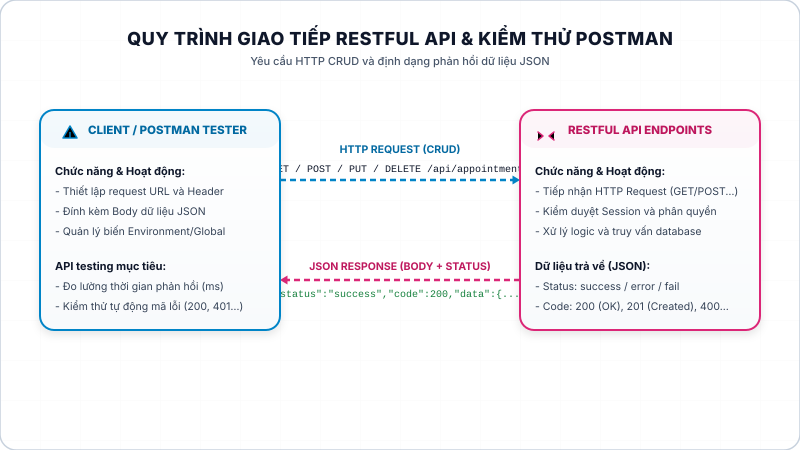
\includegraphics[width=0.9\textwidth]{restful_api_flow.svg}
    \caption{Sơ đồ luồng giao tiếp dữ liệu RESTful API qua giao thức HTTP và phản hồi JSON}
    \label{fig:restful_api_flow}
\end{figure}

\subsection{Framework Bootstrap 5.3 và Thiết kế đáp ứng (Responsive Design)}
Bootstrap 5.3 là framework CSS nguồn mở được sử dụng để phát triển nhanh các giao diện web có khả năng thích ứng hoàn hảo trên mọi kích thước màn hình thiết bị từ điện thoại đến máy tính để bàn (\textbf{Responsive Web Design}).
\begin{itemize}
    \item \textbf{Cơ chế Grid System (Hệ thống lưới):} Bootstrap chia chiều rộng giao diện thành 12 cột ảo. Bằng cách sử dụng các lớp CSS kết hợp cùng các breakpoints (điểm ngắt kích thước màn hình), lập trình viên có thể chỉ định chính xác bố cục của từng khối nội dung. Ví dụ trong Dashboard bệnh nhân, khung lọc thông tin chiếm 3 cột bên trái và danh sách bài tuyển dụng chiếm 9 cột bên phải trên máy tính, nhưng sẽ tự động co lại chiếm đủ 12 cột dọc xếp chồng lên nhau trên màn hình điện thoại nhỏ.
    \item \textbf{Các Component tiện ích:} Cung cấp các thành phần giao diện chuẩn hóa (Cards, Modals, Navbar, Alerts, Spacing, Buttons) được tối ưu hóa khả năng phản hồi trực quan, giúp tăng tốc độ thiết kế và đảm bảo tính đồng nhất thẩm mỹ cho toàn bộ hệ thống.
\end{itemize}

\section{Các công nghệ phát triển phía Server (Backend) và Cơ sở dữ liệu}

\subsection{Ngôn ngữ lập trình PHP và kiến trúc hoạt động}
PHP (Hypertext Preprocessor) là ngôn ngữ kịch bản chạy phía máy chủ (server-side) mã nguồn mở được thiết kế tối ưu cho phát triển web. PHP chạy trực tiếp trên máy chủ, cho phép xử lý các logic nghiệp vụ phức tạp, truy vấn dữ liệu từ MySQL, quản lý phiên làm việc thông qua Session/Cookie, phân quyền người dùng và tạo ra mã nguồn HTML kết quả để gửi về cho client. Trong hệ thống kết nối y tế, PHP đóng vai trò xử lý toàn bộ logic như đăng ký tài khoản, gửi tin nhắn, điều phối cuộc gọi và kết nối đến các mô hình AI.

PHP quản lý trạng thái đăng nhập của người dùng thông qua cơ chế \textbf{Session}: Server tạo một vùng nhớ tạm thời tương ứng với từng phiên làm việc của người dùng và gửi về trình duyệt một chuỗi khóa định danh duy nhất gọi là Session ID lưu trong Cookie. Trong các request tiếp theo, Cookie này được tự động gửi kèm lên server để nhận dạng danh tính và vai trò người dùng một cách an toàn.

\begin{figure}[H]
    \centering
    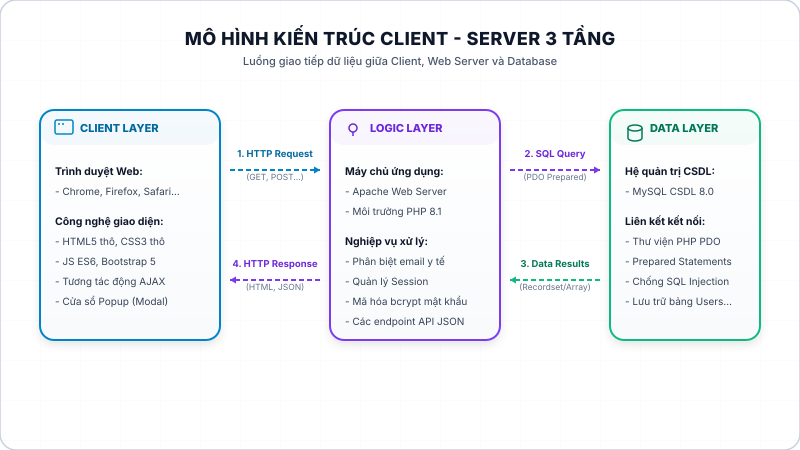
\includegraphics[width=0.9\textwidth]{client_server_3_tier.svg}
    \caption{Sơ đồ tương tác cấu trúc Client-Server 3 tầng (3-Tier Architecture) trong hệ thống}
    \label{fig:client_server_3_tier}
\end{figure}

\begin{figure}[H]
    \centering
    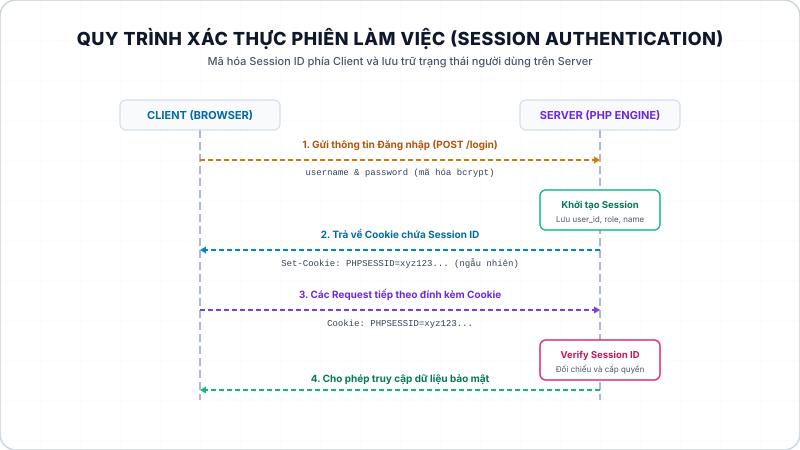
\includegraphics[width=0.9\textwidth]{session_auth_flow.svg}
    \caption{Sơ đồ tuần tự quy trình xác thực phiên làm việc (Session Authentication) giữa Client và Server}
    \label{fig:session_auth_flow}
\end{figure}

\subsection{Kết nối CSDL an toàn bằng PHP Data Objects (PDO)}
PDO là lớp giao tiếp cơ sở dữ liệu thống nhất được tích hợp sẵn trong PHP, cung cấp một giao thức trừu tượng hóa cơ sở dữ liệu chung cho phép ứng dụng kết nối tới nhiều hệ quản trị cơ sở dữ liệu khác nhau mà không cần thay đổi logic viết câu lệnh truy vấn.

Một ưu điểm bảo mật cốt lõi khi sử dụng PDO là cơ chế chuẩn bị trước câu lệnh (\textbf{Prepared Statements}) kết hợp ràng buộc tham số (\textbf{Parameter Binding}). Đây là phương pháp tối ưu nhất để phòng chống lỗ hổng bảo mật nghiêm trọng \textbf{SQL Injection}:
\begin{itemize}
    \item \textbf{Lỗ hổng SQL Injection:} Xảy ra khi lập trình viên trực tiếp nối chuỗi dữ liệu đầu vào của người dùng vào câu lệnh SQL. Kẻ tấn công có thể chèn các ký tự đặc biệt hoặc mã SQL độc hại (ví dụ: \texttt{' OR '1'='1}) qua ô nhập liệu để làm thay đổi logic câu lệnh ban đầu, truy cập hoặc xóa trái phép dữ liệu của hệ thống.
    \item \textbf{Cơ chế phòng vệ của PDO Prepared Statements:} Khi dùng prepared statements, cấu trúc của câu lệnh truy vấn SQL được biên dịch và gửi lên máy chủ MySQL trước dưới dạng bộ khung không chứa dữ liệu cụ thể (sử dụng các tham số placeholder dạng dấu chấm hỏi \texttt{?} hoặc tham số đặt tên). Sau đó, các biến dữ liệu từ người dùng mới được liên kết (\texttt{bind}) vào câu lệnh dưới dạng giá trị thô thuần túy. MySQL sẽ xử lý các tham số này chỉ dưới dạng các giá trị trường dữ liệu chứ không bao giờ biên dịch chúng thành mã SQL thực thi, từ đó loại bỏ hoàn toàn khả năng khai thác SQL Injection.
\end{itemize}

Đoạn mã cấu trúc thực tế xử lý truy vấn thông tin người dùng sử dụng PDO prepared statements trong hệ thống:
\begin{lstlisting}[language=PHP]
$stmt = $pdo->prepare("SELECT id, password_hash, role FROM users WHERE email = ? LIMIT 1");
$stmt->execute([$email]);
$user = $stmt->fetch();
\end{lstlisting}

\begin{figure}[H]
    \centering
    
\includegraphics[width=0.9\textwidth]{prepared_statements.svg}
    \caption{Sơ đồ cơ chế hoạt động của PDO Prepared Statements chống lại lỗ hổng SQL Injection}
    \label{fig:prepared_statements}
\end{figure}

\subsection{Hệ quản trị cơ sở dữ liệu quan hệ MySQL và cơ chế InnoDB}
MySQL là hệ quản trị cơ sở dữ liệu quan hệ (RDBMS) mã nguồn mở hoạt động theo mô hình bảng lưu trữ cấu trúc chặt chẽ. Dữ liệu được tổ chức thành các bảng có mối quan hệ liên kết với nhau thông qua cơ chế khóa chính (Primary Key) xác định tính duy nhất của bản ghi và khóa ngoại (Foreign Key) để đảm bảo tính toàn vẹn tham chiếu. MySQL hỗ trợ cơ chế lưu trữ an toàn, truy vấn dữ liệu hiệu năng cao và thích hợp cho các ứng dụng web động xử lý khối lượng giao dịch lớn. Trong dự án này, MySQL sử dụng công cụ lưu trữ (Storage Engine) mặc định là \textbf{InnoDB} nhờ các tính năng nâng cao như hỗ trợ ràng buộc toàn vẹn khóa ngoại (Foreign Keys) để tự động hóa kiểm tra tính nhất quán dữ liệu giữa các bảng và hỗ trợ đầy đủ các giao dịch cơ sở dữ liệu (Database Transactions) bảo đảm tính toàn vẹn dữ liệu.

Khi xử lý các nghiệp vụ nhạy cảm như tạo lịch hẹn y tế (bảng \texttt{appointments}) hay duyệt thanh toán, dữ liệu cần được ghi đồng thời vào nhiều bảng liên quan. MySQL InnoDB đảm bảo các giao dịch này tuân thủ nghiêm ngặt 4 thuộc tính \textbf{ACID}:
\begin{itemize}
    \item \textbf{Atomicity (Tính nguyên tử):} Đảm bảo một giao dịch được thực hiện trọn vẹn hoặc không thực hiện gì cả. Nếu một câu lệnh trong chuỗi giao dịch thất bại, toàn bộ giao dịch sẽ bị thu hồi (Rollback) về trạng thái ban đầu.
    \item \textbf{Consistency (Tính nhất quán):} Đảm bảo cơ sở dữ liệu chuyển đổi từ trạng thái hợp lệ này sang trạng thái hợp lệ khác sau khi giao dịch thành công, tuân thủ tất cả các ràng buộc toàn vẹn dữ liệu.
    \item \textbf{Isolation (Tính cô lập):} Đảm bảo các giao dịch chạy đồng thời độc lập với nhau, kết quả của một giao dịch đang thực thi sẽ không được nhìn thấy bởi các giao dịch khác cho đến khi nó được ghi nhận (Commit).
    \item \textbf{Durability (Tính bền vững):} Đảm bảo một khi giao dịch đã Commit thành công, các thay đổi dữ liệu sẽ được lưu trữ vĩnh viễn vào bộ nhớ lưu trữ vật lý và không bị mất ngay cả khi hệ thống xảy ra sự cố đột ngột.
\end{itemize}

\section{Công nghệ truyền thông thời gian thực WebRTC}

\subsection{Tổng quan về WebRTC (Web Real-Time Communication)}
WebRTC là một bộ tiêu chuẩn công nghệ nguồn mở cho phép các trình duyệt và ứng dụng di động thiết lập kết nối truyền tải video, audio và dữ liệu thời gian thực ngang hàng trực tiếp (Peer-to-Peer - P2P) mà không cần cài đặt plugin hay phần mềm trung gian độc lập. Ba thư viện API JavaScript nền tảng cấu thành WebRTC gồm:
\begin{itemize}
    \item \texttt{MediaStream} (\texttt{getUserMedia}): Yêu cầu quyền truy cập từ trình duyệt để kích hoạt camera và microphone của người dùng đầu cuối để thu luồng video/audio.
    \item \texttt{RTCPeerConnection}: Thành phần chính quản lý tiến trình thiết lập kết nối mạng, mã hóa luồng dữ liệu truyền phát âm thanh/hình ảnh thời gian thực, tự động thích ứng với băng thông mạng để đảm bảo chất lượng cuộc gọi tốt nhất.
    \item \texttt{RTCDataChannel}: Kênh truyền dữ liệu dạng text/binary hai chiều có độ trễ cực thấp trực tiếp giữa hai trình duyệt.
\end{itemize}

\subsection{Quy trình Signaling (Báo hiệu) và vượt tường lửa (NAT Traversal)}
Dù WebRTC truyền phát luồng dữ liệu (Stream) trực tiếp giữa hai máy khách (P2P), hai trình duyệt vẫn cần một kênh trung gian ban đầu để trao đổi địa chỉ IP công cộng và cấu hình codec trước khi kết nối trực tiếp được thiết lập. Kênh này gọi là máy chủ Signaling (Signaling Server).
\begin{itemize}
    \item \textbf{Luồng bắt tay Signaling:}
    \begin{enumerate}
        \item Thiết bị gọi (Caller) khởi tạo một gói mô tả SDP (Session Description Protocol) gọi là \textbf{Offer} chứa thông tin cấu hình phần cứng của mình. Gói Offer này được gửi lên máy chủ Signaling.
        \item Máy chủ Signaling chuyển gói Offer này tới thiết bị nhận (Callee).
        \item Callee nhận Offer, tạo một gói phản hồi SDP tương ứng gọi là \textbf{Answer} và gửi lại qua máy chủ Signaling để chuyển tiếp tới Caller.
        \item Đồng thời, hai trình duyệt liên tục thu thập địa chỉ mạng của mình gọi là các gói \textbf{ICE Candidates} và trao đổi chéo cho nhau qua máy chủ báo hiệu để tìm ra lộ trình bắt tay vật lý khả thi.
    \end{enumerate}
    \item \textbf{Hạ tầng vượt tường lửa NAT với STUN/TURN và ICE:}
    Đa số người dùng Internet cá nhân đều nằm sau các router NAT hoặc hệ thống tường lửa (Firewall), khiến địa chỉ IP nội bộ không thể truy cập trực tiếp từ bên ngoài. WebRTC giải quyết thách thức này qua khung giao thức ICE (Interactive Connectivity Establishment) kết hợp các máy chủ hỗ trợ:
    \begin{itemize}
        \item \textbf{STUN (Session Traversal Utilities for NAT):} Máy chủ trung gian giúp trình duyệt tự khám phá ra địa chỉ IP công cộng và cổng mở của chính nó để đóng gói gửi cho đối phương.
        \item \textbf{TURN (Traversal Using Relays around NAT):} Trong trường hợp cả hai thiết bị đều nằm sau lớp NAT đối xứng phức tạp không thể kết nối trực tiếp, TURN Server đóng vai trò máy chủ trung chuyển (Relay) luồng video/audio. Mặc dù làm mất đi tính chất P2P thuần túy, TURN đảm bảo cuộc gọi luôn được thiết lập thành công trong mọi điều kiện mạng.
    \end{itemize}
\end{itemize}

\begin{figure}[H]
    \centering
    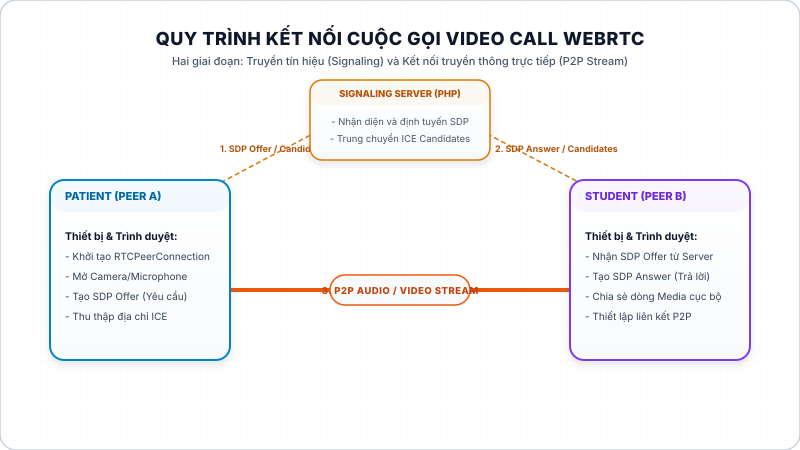
\includegraphics[width=0.9\textwidth]{webrtc_flow.svg}
    \caption{Sơ đồ luồng tín hiệu báo hiệu (Signaling) và thiết lập kết nối WebRTC P2P}
    \label{fig:webrtc_flow}
\end{figure}

\subsection{Cơ chế Signaling qua Cơ sở dữ liệu (Database-based Signaling)}
Trong dự án này, để tối ưu hóa khả năng triển khai trên các môi trường hosting PHP Apache phổ thông mà không cần duy trì các máy chủ WebSockets (Node.js) đắt đỏ, hệ thống triển khai giải pháp Signaling qua cơ sở dữ liệu kết hợp AJAX Polling:
\begin{itemize}
    \item Gói tín hiệu Offer, Answer, và các gói ICE Candidates từ client gửi lên backend qua AJAX POST và được lưu trữ trực tiếp vào bảng cơ sở dữ liệu \texttt{call_signals}.
    \item Trình duyệt phía người nhận sử dụng Javascript gửi yêu cầu kiểm tra định kỳ (HTTP GET Polling sau mỗi 1.5 - 2 giây) tới tệp \texttt{call_signaling.php} để dò tìm tín hiệu báo hiệu mới. Khi có tín hiệu, trình duyệt lập tức nạp gói tin SDP và ICE vào luồng xử lý WebRTC để bắt đầu cuộc gọi.
\end{itemize}

\section{Trí tuệ nhân tạo tạo sinh Generative AI và Tích hợp API}

\subsection{Trợ lý y tế ảo dựa trên mô hình ngôn ngữ lớn (LLM)}
Generative AI (Trí tuệ nhân tạo tạo sinh) đại diện cho bước đột phá lớn của học máy, cho phép tạo ra văn bản tự nhiên giống con người dựa trên kiến trúc mạng nơ-ron Transformer với cơ chế chú ý tự động (Self-Attention mechanism). Mô hình ngôn ngữ lớn (LLM) được huấn luyện trước trên tập dữ liệu khổng lồ giúp trợ lý ảo y tế trên website có thể hiểu ngữ cảnh câu hỏi, trả lời các thắc mắc kiến thức sức khỏe thông dụng của bệnh nhân, hướng dẫn các kỹ năng lâm sàng cho sinh viên, đồng thời hỗ trợ vận hành hệ thống một cách tối ưu.

\subsection{Google Gemini API và kỹ thuật xây dựng rào cản an toàn y tế}
Google cung cấp dịch vụ đám mây cho phép kết nối trực tiếp tới mô hình AI tiên tiến \texttt{gemini-2.5-flash} qua cổng API RESTful để thực hiện phản hồi thông minh với tốc độ xử lý nhanh và độ hiểu biết cao.
\begin{itemize}
    \item \textbf{Kỹ thuật Prompt Engineering và System Instruction:} Thiết lập chỉ thị hệ thống trước khi bắt đầu hội thoại là kỹ thuật thiết yếu để cấu hình hành vi cho AI. Trong hệ thống kết nối y tế, một hệ thống chỉ thị (Prompt Instruction) nghiêm ngặt được thiết lập trong tệp \texttt{api/ai_gemini.php} để xây dựng rào cản an toàn (Guardrails) y tế cho người dùng:
    \begin{itemize}
        \item \textbf{Lọc chủ đề (Topic Control):} AI tự động từ chối trả lời mọi câu hỏi không thuộc chủ đề y học, chăm sóc sức khỏe và hướng dẫn sử dụng website (như yêu cầu làm toán, kể chuyện, viết code lập trình).
        \item \textbf{Ngăn chặn tự chẩn đoán và kê đơn:} AI bị cấm chỉ định liều lượng thuốc hay khẳng định chắc chắn chẩn đoán bệnh cụ thể. Chỉ được cung cấp thông tin tham khảo về triệu chứng và khuyên dùng các nhóm thuốc hạ sốt, bù nước cơ bản.
        \item \textbf{Giao thức triệu chứng nguy kịch (Red Flags Protocol):} Khi phát hiện các triệu chứng nguy cấp (đau thắt ngực, khó thở nghiêm trọng, co giật, liệt méo miệng đột ngột), AI lập tức dừng tư vấn y tế thông thường và bắt buộc hiển thị cảnh báo khẩn cấp hướng dẫn người bệnh gọi ngay cấp cứu 115.
    \end{itemize}
\end{itemize}

\subsection{Hugging Face Inference API và Cơ chế dự phòng chịu lỗi (Fallback)}
Để đảm bảo trợ lý y tế ảo hoạt động liên tục 24/7 khi Google Gemini gặp các sự cố như hết hạn ngạch API miễn phí, quá tải máy chủ hoặc mất kết nối mạng, hệ thống được trang bị cơ chế chịu lỗi (Fault Tolerance):
\begin{itemize}
    \item \textbf{Hugging Face Inference API:} Cho phép gửi truy vấn trực tiếp đến mô hình chatbot nguồn mở gọn nhẹ như \texttt{Meta BlenderBot-400M-distill} chạy trên đám mây Hugging Face.
    \item \textbf{Luồng xử lý dự phòng:} Backend PHP được viết trong khối lệnh \texttt{try-catch}. Khi lời gọi API Gemini xảy ra lỗi hoặc trả về mã trạng thái thất bại, hệ thống lập tức bắt ngoại lệ này và thực hiện cuộc gọi dự phòng tới Hugging Face API để lấy câu trả lời. Nếu cả hai dịch vụ API đám mây đều mất kết nối, hệ thống sẽ gọi hàm phân tích từ khóa nội bộ \texttt{getLocalFallbackResponse()} để đưa ra phản hồi y tế/vận hành định sẵn phù hợp.
\end{itemize}

\begin{figure}[H]
    \centering
    
\includegraphics[width=0.9\textwidth]{ai_fallback_flow.svg}
    \caption{Sơ đồ luồng dự phòng chịu lỗi (AI Fallback \& Local Fallback Flow) của trợ lý ảo}
    \label{fig:ai_fallback_flow}
\end{figure}

\section{Công nghệ đóng gói và triển khai Container Docker}

\subsection{Công nghệ Containerization và ảo hóa cấp độ hệ điều hành}
Containerization là công nghệ đóng gói toàn bộ mã nguồn ứng dụng, tệp cấu hình môi trường và các thư viện liên quan thành một khối đóng kín độc lập gọi là Container.
\begin{itemize}
    \item \textbf{Sự cách biệt với Máy ảo (Virtual Machine - VM):} Máy ảo hoạt động dựa trên phần mềm Hypervisor để giả lập phần cứng và yêu cầu chạy một hệ điều hành khách (Guest OS) riêng biệt bên trong. Việc này chiếm dụng lượng tài nguyên phần cứng rất lớn (vài GB ổ cứng, RAM) và khởi động chậm. Trái lại, các Container dùng chung nhân của hệ điều hành máy chủ (Host OS) và được cô lập về tài nguyên ở tầng nhân hệ điều hành thông qua hai cơ chế lõi của Linux Kernel là \textbf{namespaces} (cô lập tài nguyên mạng, tiến trình, đĩa cứng) và \textbf{cgroups} (giới hạn phần cứng RAM/CPU), giúp dung lượng container cực kỳ nhẹ (chỉ vài chục MB), khởi động tức thì và tiết kiệm tối đa RAM/CPU.
\end{itemize}

\begin{figure}[H]
    \centering
    
\includegraphics[width=0.9\textwidth]{docker_vs_vm.svg}
    \caption{Sơ đồ so sánh kiến trúc giữa máy ảo Virtual Machine và Docker Container}
    \label{fig:docker_vs_vm}
\end{figure}

\subsection{Môi trường ảo hóa với Docker và Docker Compose}
\begin{itemize}
    \item \textbf{Docker Image và Container:} Docker Image là khuôn mẫu tĩnh chứa toàn bộ môi trường và mã nguồn đã đóng gói. Docker Container là trạng thái thực thi trực tiếp của ảnh tĩnh đó. Quy trình biên dịch ảnh tĩnh này được đặc tả chi tiết trong tệp cấu hình \texttt{Dockerfile} (tải hệ điều hành Alpine nhẹ, cài đặt Apache, PHP 8.2 và các extension PDO).
    \item \textbf{Docker Compose:} Công cụ hỗ trợ chạy các hệ thống đa container. Thông qua tệp cấu hình \texttt{docker-compose.yml}, lập trình viên thiết lập mạng nội bộ liên kết đồng bộ hai container chạy song song: một Web Server chứa mã nguồn PHP và một MySQL Server chứa CSDL. Docker Compose đảm bảo môi trường phát triển của lập trình viên và môi trường chấm đồ án của giảng viên luôn đồng nhất tuyệt đối, tránh lỗi "chạy được trên máy em nhưng lỗi trên máy khác".
\end{itemize}


% ==================== CHƯƠNG 3: HIỆN THỰC HÓA NGHIÊN CỨU ====================
\chapter{HIỆN THỰC HÓA NGHIÊN CỨU}

\section{Phân tích yêu cầu hệ thống}

\subsection{Yêu cầu chức năng}

\subsubsection{Đối với Bệnh nhân}
\begin{itemize}
    \item Đăng ký tài khoản với vai trò bệnh nhân
    \item Đăng nhập/Đăng xuất
    \item Xem danh sách tin ứng tuyển của sinh viên
    \item Đăng tin tuyển dụng người chăm sóc
    \item Tìm kiếm, lọc tin theo khu vực, danh mục
    \item Lưu tin yêu thích
    \item Gửi tin nhắn cho sinh viên
    \item Đánh giá sinh viên sau khi sử dụng dịch vụ
    \item Quản lý hồ sơ cá nhân
\end{itemize}

\subsubsection{Đối với Sinh viên Y khoa}
\begin{itemize}
    \item Đăng ký tài khoản với vai trò sinh viên
    \item Xác thực tài khoản bằng thẻ sinh viên
    \item Xem danh sách tin tuyển dụng
    \item Đăng tin ứng tuyển (sau khi được xác thực)
    \item Xin cấp quyền đăng tin
    \item Gửi tin nhắn cho bệnh nhân
    \item Quản lý hồ sơ cá nhân
    \item Xem lịch sử nhận việc
\end{itemize}

\subsubsection{Đối với Quản trị viên}
\begin{itemize}
    \item Quản lý người dùng (xem, khóa, xóa)
    \item Quản lý bài viết (duyệt, ẩn, xóa)
    \item Xử lý yêu cầu xác thực sinh viên
    \item Xử lý yêu cầu cấp quyền đăng tin
    \item Xem và xử lý báo cáo vi phạm
    \item Gửi thông báo đến người dùng
    \item Xem thống kê hệ thống
\end{itemize}

\subsection{Yêu cầu phi chức năng}
\begin{itemize}
    \item Giao diện thân thiện, dễ sử dụng
    \item Tương thích với nhiều trình duyệt
    \item Responsive trên các thiết bị
    \item Bảo mật thông tin người dùng
    \item Thời gian phản hồi nhanh
\end{itemize}

\section{Thiết kế hệ thống}

\subsection{Biểu đồ Use Case}

Biểu đồ Use Case mô tả các chức năng chính của hệ thống và các tác nhân tương tác.

\begin{figure}[H]
    \centering
    \includegraphics[width=0.9\textwidth]{usecase.png}
    \caption{Biểu đồ Use Case tổng quan hệ thống}
    \label{fig:usecase}
\end{figure}

\textbf{Các tác nhân (Actors):}
\begin{itemize}
    \item \textbf{Khách (Guest):} Người dùng chưa đăng nhập
    \item \textbf{Bệnh nhân (Patient):} Người dùng có nhu cầu tìm người chăm sóc
    \item \textbf{Sinh viên (Student):} Sinh viên Y khoa muốn tìm việc
    \item \textbf{Quản trị viên (Admin):} Người quản lý hệ thống
\end{itemize}

\subsection{Thiết kế cơ sở dữ liệu}

\subsubsection{Biểu đồ ERD}

\begin{figure}[H]
    \centering
    \includegraphics[width=0.95\textwidth]{ERD.png}
    \caption{Biểu đồ ERD - Quan hệ thực thể}
    \label{fig:erd}
\end{figure}

\subsubsection{Mô tả các bảng dữ liệu}

\begin{table}[H]
\centering
\caption{Bảng Users - Thông tin người dùng}
\begin{tabular}{|l|l|l|}
\hline
\textbf{Tên trường} & \textbf{Kiểu dữ liệu} & \textbf{Mô tả} \\
\hline
id & INT (PK) & Mã người dùng \\
name & VARCHAR(150) & Họ tên \\
email & VARCHAR(255) & Email (unique) \\
password & VARCHAR(255) & Mật khẩu (hash) \\
role & ENUM & Vai trò (patient/student) \\
bio & TEXT & Giới thiệu bản thân \\
location & VARCHAR(255) & Địa chỉ \\
phone & VARCHAR(50) & Số điện thoại \\
verified & TINYINT & Trạng thái xác thực SV \\
is\_admin & TINYINT & Quyền admin \\
can\_post & TINYINT & Quyền đăng tin \\
created\_at & TIMESTAMP & Ngày tạo \\
\hline
\end{tabular}
\end{table}

\begin{table}[H]
\centering
\caption{Bảng Posts - Bài đăng}
\begin{tabular}{|l|l|l|}
\hline
\textbf{Tên trường} & \textbf{Kiểu dữ liệu} & \textbf{Mô tả} \\
\hline
id & INT (PK) & Mã bài đăng \\
user\_id & INT (FK) & Mã người đăng \\
title & VARCHAR(255) & Tiêu đề \\
content & TEXT & Nội dung \\
type & ENUM & Loại (recruitment/application) \\
category & VARCHAR(100) & Danh mục \\
area & VARCHAR(255) & Khu vực \\
contact\_info & VARCHAR(255) & Thông tin liên hệ \\
suggested\_price & INT & Giá đề xuất \\
status & ENUM & Trạng thái (open/taken/closed) \\
created\_at & TIMESTAMP & Ngày tạo \\
\hline
\end{tabular}
\end{table}

\begin{table}[H]
\centering
\caption{Bảng Messages - Tin nhắn}
\begin{tabular}{|l|l|l|}
\hline
\textbf{Tên trường} & \textbf{Kiểu dữ liệu} & \textbf{Mô tả} \\
\hline
id & INT (PK) & Mã tin nhắn \\
from\_user & INT (FK) & Người gửi \\
to\_user & INT (FK) & Người nhận \\
post\_id & INT (FK) & Bài đăng liên quan \\
message & TEXT & Nội dung tin nhắn \\
created\_at & TIMESTAMP & Thời gian gửi \\
\hline
\end{tabular}
\end{table}

\section{Cài đặt hệ thống}

\subsection{Cấu trúc thư mục dự án}

\begin{verbatim}
DACN1/
├── assets/
│   ├── css/
│   │   └── style.css
│   └── js/
├── uploads/
├── config.php
├── header.php
├── footer.php
├── index.php
├── login.php
├── register.php
├── dashboard_patient.php
├── dashboard_student.php
├── create_recruitment.php
├── create_application.php
├── view_post.php
├── chat.php
├── conversations.php
├── admin_dashboard.php
├── admin_users.php
├── admin_posts.php
├── admin_verifications.php
├── admin_reports.php
└── database.sql
\end{verbatim}

\subsection{Cấu hình kết nối cơ sở dữ liệu}

File \texttt{config.php} chứa thông tin kết nối database:

\begin{lstlisting}[language=PHP]
<?php
define('DB_HOST', '127.0.0.1');
define('DB_NAME', 'dacn1_db');
define('DB_USER', 'root');
define('DB_PASS', '');

$pdo = new PDO(
    'mysql:host='.DB_HOST.';dbname='.DB_NAME,
    DB_USER, DB_PASS,
    [PDO::ATTR_ERRMODE => PDO::ERRMODE_EXCEPTION]
);
\end{lstlisting}

\subsection{Xử lý đăng ký và phân quyền}

Hệ thống tự động phân quyền dựa trên email:
\begin{itemize}
    \item Email kết thúc bằng \texttt{edu.vn} $\rightarrow$ Vai trò: Sinh viên
    \item Email khác $\rightarrow$ Vai trò: Bệnh nhân
\end{itemize}

\subsection{Xác thực sinh viên}

Quy trình xác thực sinh viên:
\begin{enumerate}
    \item Sinh viên gửi yêu cầu xác thực kèm ảnh thẻ sinh viên
    \item Admin xem xét và duyệt/từ chối yêu cầu
    \item Nếu được duyệt, sinh viên có thể đăng tin ứng tuyển
\end{enumerate}

\subsection{Hệ thống tin nhắn}

Hệ thống hỗ trợ nhắn tin trực tiếp giữa người dùng:
\begin{itemize}
    \item Tạo cuộc hội thoại mới khi nhắn tin lần đầu
    \item Lưu trữ lịch sử tin nhắn
    \item Hiển thị trạng thái online của người dùng
\end{itemize}


% ==================== CHƯƠNG 4: KẾT QUẢ NGHIÊN CỨU ====================
\chapter{KẾT QUẢ NGHIÊN CỨU}

\section{Giao diện người dùng}

\subsection{Trang chủ}

Trang chủ hiển thị danh sách các tin đăng mới nhất, cho phép người dùng tìm kiếm và lọc theo danh mục, khu vực.

\begin{figure}[H]
    \centering
    \includegraphics[width=0.9\textwidth]{{Giao diện trang chủ}.png}
    \caption{Giao diện trang chủ}
    \label{fig:trangchu}
\end{figure}

\subsection{Đăng ký và Đăng nhập}

\begin{figure}[H]
    \centering
    \includegraphics[width=0.8\textwidth]{{Giao diện đăng kí}.png}
    \caption{Giao diện đăng ký tài khoản}
    \label{fig:dangky}
\end{figure}

\begin{figure}[H]
    \centering
    \includegraphics[width=0.8\textwidth]{{Giao diện đăng nhập}.png}
    \caption{Giao diện đăng nhập}
    \label{fig:dangnhap}
\end{figure}

\subsection{Trang Bệnh nhân}

\subsubsection{Bảng điều khiển}

\begin{figure}[H]
    \centering
    \includegraphics[width=0.9\textwidth]{{Giao diện bảng điều khiển trang bệnh nhân}.png}
    \caption{Bảng điều khiển trang bệnh nhân}
    \label{fig:dashboard_patient}
\end{figure}

\subsubsection{Đánh giá sinh viên}

\begin{figure}[H]
    \centering
    \includegraphics[width=0.8\textwidth]{{Giao diện đánh giá trang bệnh nhân}.png}
    \caption{Giao diện đánh giá sinh viên}
    \label{fig:rating}
\end{figure}

\subsubsection{Lịch sử nhận việc}

\begin{figure}[H]
    \centering
    \includegraphics[width=0.9\textwidth]{{Giao diện lịch sử nhận việc trang bệnh nhân}.png}
    \caption{Giao diện lịch sử nhận việc - Bệnh nhân}
    \label{fig:history_patient}
\end{figure}

\subsection{Trang Sinh viên}

\subsubsection{Bảng điều khiển}

\begin{figure}[H]
    \centering
    \includegraphics[width=0.9\textwidth]{{Giao diện bảng điều khiển trang sinh viên}.png}
    \caption{Bảng điều khiển trang sinh viên}
    \label{fig:dashboard_student}
\end{figure}

\subsubsection{Cập nhật hồ sơ}

\begin{figure}[H]
    \centering
    \includegraphics[width=0.8\textwidth]{{Giao diện form cập nhật hồ sơ trang sinh viên}.png}
    \caption{Form cập nhật hồ sơ sinh viên}
    \label{fig:update_profile}
\end{figure}

\subsubsection{Xin xác thực và cấp quyền đăng tin}

\begin{figure}[H]
    \centering
    \includegraphics[width=0.8\textwidth]{{Giao diện form xin xác thực tài khoản}.png}
    \caption{Form xin xác thực tài khoản}
    \label{fig:request_verify}
\end{figure}

\begin{figure}[H]
    \centering
    \includegraphics[width=0.8\textwidth]{{Giao diện form xin cấp quyền đăng tin}.png}
    \caption{Form xin cấp quyền đăng tin}
    \label{fig:request_post}
\end{figure}

\subsubsection{Lịch sử nhận việc}

\begin{figure}[H]
    \centering
    \includegraphics[width=0.9\textwidth]{{Giao diện lịch sử nhận việc trang sinh viên}.png}
    \caption{Lịch sử nhận việc - Sinh viên}
    \label{fig:history_student}
\end{figure}

\subsection{Chức năng chung}

\subsubsection{Hội thoại và Tin nhắn}

\begin{figure}[H]
    \centering
    \includegraphics[width=0.9\textwidth]{{Giao diện hội thoại}.png}
    \caption{Giao diện hội thoại}
    \label{fig:chat}
\end{figure}

\subsubsection{Bạn bè}

\begin{figure}[H]
    \centering
    \includegraphics[width=0.9\textwidth]{{Giao diện trang bạn bè}.png}
    \caption{Giao diện trang bạn bè}
    \label{fig:friends}
\end{figure}

\subsubsection{Yêu thích}

\begin{figure}[H]
    \centering
    \includegraphics[width=0.9\textwidth]{{Giao diện trang bài tuyển yêu thích}.png}
    \caption{Giao diện bài tuyển yêu thích}
    \label{fig:favorites}
\end{figure}

\subsubsection{Hỗ trợ tài khoản}

\begin{figure}[H]
    \centering
    \includegraphics[width=0.9\textwidth]{{Giao diện trang hỗ trợ tài khoản}.png}
    \caption{Giao diện hỗ trợ tài khoản}
    \label{fig:support}
\end{figure}

\subsection{Trang Quản trị}

\subsubsection{Bảng điều khiển Admin}

\begin{figure}[H]
    \centering
    \includegraphics[width=0.9\textwidth]{{Giao diện bảng điều khiển trang quản trị}.png}
    \caption{Bảng điều khiển trang quản trị}
    \label{fig:admin_dashboard}
\end{figure}

\subsubsection{Quản lý người dùng}

\begin{figure}[H]
    \centering
    \includegraphics[width=0.9\textwidth]{{Giao diện quản lý người dùng}.png}
    \caption{Giao diện quản lý người dùng}
    \label{fig:admin_users}
\end{figure}

\subsubsection{Quản lý bài viết}

\begin{figure}[H]
    \centering
    \includegraphics[width=0.9\textwidth]{{Giao diện quản lý bài viết}.png}
    \caption{Giao diện quản lý bài viết}
    \label{fig:admin_posts}
\end{figure}

\subsubsection{Quản lý tin đăng}

\begin{figure}[H]
    \centering
    \includegraphics[width=0.9\textwidth]{{Giao diện đăng tin tuyển trang quản trị}.png}
    \caption{Quản lý tin tuyển dụng}
    \label{fig:admin_recruitment}
\end{figure}

\begin{figure}[H]
    \centering
    \includegraphics[width=0.9\textwidth]{{Giao diện đăng tin ứng tuyển trang quản trị}.png}
    \caption{Quản lý tin ứng tuyển}
    \label{fig:admin_application}
\end{figure}

\subsubsection{Gửi thông báo}

\begin{figure}[H]
    \centering
    \includegraphics[width=0.8\textwidth]{{Giao dện gửi thông báo }.png}
    \caption{Giao diện gửi thông báo}
    \label{fig:admin_notify}
\end{figure}


\section{Đánh giá kết quả}

\subsection{Các chức năng đã hoàn thành}

\begin{table}[H]
\centering
\caption{Bảng đánh giá các chức năng}
\begin{tabular}{|c|l|c|}
\hline
\textbf{STT} & \textbf{Chức năng} & \textbf{Trạng thái} \\
\hline
1 & Đăng ký/Đăng nhập & Hoàn thành \\
2 & Phân quyền người dùng & Hoàn thành \\
3 & Đăng tin tuyển dụng & Hoàn thành \\
4 & Đăng tin ứng tuyển & Hoàn thành \\
5 & Tìm kiếm, lọc tin & Hoàn thành \\
6 & Lưu tin yêu thích & Hoàn thành \\
7 & Hệ thống tin nhắn & Hoàn thành \\
8 & Xác thực sinh viên & Hoàn thành \\
9 & Đánh giá người dùng & Hoàn thành \\
10 & Báo cáo vi phạm & Hoàn thành \\
11 & Quản lý người dùng (Admin) & Hoàn thành \\
12 & Quản lý bài viết (Admin) & Hoàn thành \\
13 & Xử lý xác thực (Admin) & Hoàn thành \\
14 & Gửi thông báo (Admin) & Hoàn thành \\
15 & Kết bạn & Hoàn thành \\
\hline
\end{tabular}
\end{table}

\subsection{Ưu điểm}
\begin{itemize}
    \item Giao diện thân thiện, dễ sử dụng
    \item Phân quyền rõ ràng giữa các loại người dùng
    \item Hệ thống xác thực sinh viên đảm bảo độ tin cậy
    \item Chức năng tìm kiếm, lọc hiệu quả
    \item Hệ thống tin nhắn hoạt động tốt
\end{itemize}

\subsection{Hạn chế}
\begin{itemize}
    \item Chưa có ứng dụng mobile
    \item Chưa tích hợp thanh toán trực tuyến
    \item Chưa có chức năng thông báo real-time
    \item Chưa triển khai trên server thực tế
\end{itemize}

% ==================== CHƯƠNG 5: KẾT LUẬN VÀ HƯỚNG PHÁT TRIỂN ====================
\chapter{KẾT LUẬN VÀ HƯỚNG PHÁT TRIỂN}

\section{Kết luận}

Sau quá trình nghiên cứu và thực hiện, đồ án "Xây dựng Website kết nối y tế giữa bệnh nhân và sinh viên Y khoa" đã đạt được các kết quả sau:

\subsection{Về mặt lý thuyết}
\begin{itemize}
    \item Nắm vững kiến thức về phát triển web với PHP và MySQL
    \item Hiểu rõ quy trình phân tích, thiết kế và xây dựng hệ thống thông tin
    \item Áp dụng được các mô hình UML trong thiết kế phần mềm
    \item Hiểu về bảo mật web cơ bản
\end{itemize}

\subsection{Về mặt thực tiễn}
\begin{itemize}
    \item Xây dựng thành công website với đầy đủ chức năng cơ bản
    \item Hệ thống phân quyền hoạt động chính xác
    \item Giao diện thân thiện, responsive
    \item Hệ thống xác thực sinh viên đảm bảo độ tin cậy
    \item Các chức năng tìm kiếm, nhắn tin, đánh giá hoạt động tốt
\end{itemize}

\subsection{Những đóng góp của đồ án}
\begin{itemize}
    \item Tạo ra nền tảng kết nối giữa bệnh nhân và sinh viên Y khoa
    \item Giúp bệnh nhân dễ dàng tìm được người chăm sóc phù hợp với chi phí hợp lý
    \item Tạo cơ hội thực hành và thu nhập cho sinh viên Y khoa
    \item Góp phần giải quyết vấn đề thiếu hụt nhân lực y tế tại cộng đồng
\end{itemize}

\section{Hướng phát triển}

Để hoàn thiện và mở rộng hệ thống, các hướng phát triển trong tương lai bao gồm:

\subsection{Về chức năng}
\begin{itemize}
    \item Phát triển ứng dụng mobile (Android/iOS)
    \item Tích hợp thanh toán trực tuyến
    \item Thêm chức năng thông báo real-time (WebSocket)
    \item Tích hợp video call cho tư vấn từ xa
    \item Thêm chức năng đặt lịch hẹn
    \item Xây dựng hệ thống AI chatbot hỗ trợ người dùng
\end{itemize}

\subsection{Về kỹ thuật}
\begin{itemize}
    \item Triển khai trên server thực tế (cloud hosting)
    \item Tối ưu hóa hiệu suất và bảo mật
    \item Áp dụng framework PHP (Laravel) để dễ bảo trì
    \item Sử dụng CDN cho tài nguyên tĩnh
    \item Implement caching để tăng tốc độ
\end{itemize}

\subsection{Về nghiệp vụ}
\begin{itemize}
    \item Mở rộng đối tượng người dùng (điều dưỡng, bác sĩ)
    \item Hợp tác với các trường Y khoa
    \item Liên kết với bệnh viện, phòng khám
    \item Xây dựng hệ thống đào tạo trực tuyến cho sinh viên
\end{itemize}

% ==================== TÀI LIỆU THAM KHẢO ====================
\newpage
\addcontentsline{toc}{chapter}{DANH MỤC TÀI LIỆU THAM KHẢO}
\begin{center}
\textbf{\Large DANH MỤC TÀI LIỆU THAM KHẢO}
\end{center}
\vspace{1cm}

\begin{enumerate}[label={[\arabic*]}]
    \item PHP Documentation. (2024). \textit{PHP Manual}. https://www.php.net/manual/en/
    
    \item MySQL Documentation. (2024). \textit{MySQL 8.0 Reference Manual}. https://dev.mysql.com/doc/refman/8.0/en/
    
    \item Bootstrap Team. (2024). \textit{Bootstrap Documentation}. https://getbootstrap.com/docs/
    
    \item W3Schools. (2024). \textit{HTML Tutorial}. https://www.w3schools.com/html/
    
    \item W3Schools. (2024). \textit{CSS Tutorial}. https://www.w3schools.com/css/
    
    \item Mozilla Developer Network. (2024). \textit{JavaScript Guide}. https://developer.mozilla.org/en-US/docs/Web/JavaScript/Guide
    
    \item Apache Friends. (2024). \textit{XAMPP Documentation}. https://www.apachefriends.org/
    
    \item Nguyễn Văn A. (2023). \textit{Giáo trình Phát triển ứng dụng Web}. NXB Đại học Quốc gia.
    
    \item Trần Văn B. (2022). \textit{Phân tích và thiết kế hệ thống thông tin}. NXB Giáo dục.
    
    \item Object Management Group. (2024). \textit{UML Specification}. https://www.omg.org/spec/UML/
\end{enumerate}

% ==================== PHỤ LỤC ====================
\newpage
\addcontentsline{toc}{chapter}{PHỤ LỤC}
\begin{center}
\textbf{\Large PHỤ LỤC}
\end{center}
\vspace{1cm}

\section*{Phụ lục A: Hướng dẫn cài đặt}

\subsection*{Yêu cầu hệ thống}
\begin{itemize}
    \item XAMPP (Apache + PHP + MySQL) phiên bản 7.4 trở lên
    \item Trình duyệt web hiện đại (Chrome, Firefox, Edge)
    \item Hệ điều hành: Windows 10/11
\end{itemize}

\subsection*{Các bước cài đặt}
\begin{enumerate}
    \item Cài đặt XAMPP từ https://www.apachefriends.org/
    \item Copy thư mục dự án vào \texttt{C:\textbackslash xampp\textbackslash htdocs\textbackslash DACN1}
    \item Khởi động Apache và MySQL trong XAMPP Control Panel
    \item Mở phpMyAdmin: http://localhost/phpmyadmin
    \item Tạo database mới với tên \texttt{dacn1\_db}
    \item Import file \texttt{database.sql}
    \item Cấu hình file \texttt{config.php} nếu cần
    \item Truy cập http://localhost/DACN1
\end{enumerate}

\subsection*{Tài khoản mặc định}
\begin{itemize}
    \item Admin: Tạo qua file \texttt{create\_admin.php}
    \item Người dùng: Đăng ký qua trang \texttt{register.php}
\end{itemize}

\section*{Phụ lục B: Danh sách các file chính}

\begin{table}[H]
\centering
\begin{tabular}{|l|l|}
\hline
\textbf{File} & \textbf{Mô tả} \\
\hline
config.php & Cấu hình database và hàm tiện ích \\
header.php & Header chung cho các trang \\
footer.php & Footer chung cho các trang \\
index.php & Trang chủ, danh sách tin \\
login.php & Đăng nhập \\
register.php & Đăng ký \\
logout.php & Đăng xuất \\
dashboard\_patient.php & Trang bệnh nhân \\
dashboard\_student.php & Trang sinh viên \\
create\_recruitment.php & Tạo tin tuyển dụng \\
create\_application.php & Tạo tin ứng tuyển \\
view\_post.php & Xem chi tiết tin \\
chat.php & Nhắn tin \\
conversations.php & Danh sách hội thoại \\
friends.php & Quản lý bạn bè \\
favorites.php & Tin yêu thích \\
profile.php & Hồ sơ cá nhân \\
edit\_profile.php & Chỉnh sửa hồ sơ \\
request\_verification.php & Xin xác thực \\
request\_posting\_permission.php & Xin quyền đăng tin \\
admin\_dashboard.php & Trang quản trị \\
admin\_users.php & Quản lý người dùng \\
admin\_posts.php & Quản lý bài viết \\
admin\_verifications.php & Xử lý xác thực \\
admin\_reports.php & Xem báo cáo \\
admin\_send\_notification.php & Gửi thông báo \\
\hline
\end{tabular}
\end{table}

\end{document}
